%%%%%%%%%%%%%%%%%%%%%%%%%%%%%%%%%%%%%%%%	
\subsection{PA2AM: (2-)Atomicity 一致性维护与量化}

%%%%%%%%%%%%%%%
\begin{frame}{PA2AM 工作在技术框架中的位置}
  \fig{width = 0.50\textwidth}{figures/3d-framework-pa2am.pdf}{PA2AM --- (2-)Atomicity 一致性维护与量化.}
\end{frame}
%%%%%%%%%%%%%%%
\begin{frame}{研究动机}
  \question{问题: 为什么提出 probabilistically-atomic 2-atomicity {\small (PA2AM)} 一致性?}
  \vspace{0.20cm}

  \pause
  ``数据一致性/访问延迟'' PACELC 权衡 \citeinbeamer{Abadi}{IEEE Computer}{12}:

  \fignocaption{width = 0.35\textwidth}{figures/stronger-consistency-tradeoff.pdf}

  % \begin{quote}
  %   ``As soon as a distributed storage system replicates data, a \textcolor{brown}{tradeoff 
  %   between consistency and latency} arises.''
  % \end{quote}

  \pause

  ``低延迟''至关重要:
  \begin{itemize}
	\item 100ms 额外延迟 $\Rightarrow$ 1\% 销售下滑 \href{http://glinden.blogspot.com/2006/11/marissa-mayer-at-web-20.html}{\citeinbeamer{Amazon}{Blog}{06}}
	\item 100$\sim$400ms 额外延迟 $\Rightarrow$ 0.2\%$\sim$0.6\% 搜索量下降 \href{Speed Matters for Google Web Search}{\citeinbeamer{Google}{Blog}{09}}
  \end{itemize}

  % {\small
  % \begin{table}
  %   \begin{tabular}{c|c}
  %     \textcolor{blue}{\bf 系统} & \textcolor{blue}{\bf 一致性}		\\ \hline
  %     Dynamo@Amazon \citeinbeamer{Amazon}{SOSP}{07} & eventual consistency \\ \hline
  %     PNUTS@Yahoo! \citeinbeamer{Yahoo!}{PVLDB}{08} & cache consistency \\ \hline
  %     Tao@Facebook \citeinbeamer{Facebook}{ATC}{13} & $\le$ read-after-write \\ \hline
  %   \end{tabular}
  % \end{table}
  % }
\end{frame}
%%%%%%%%%%%%%%%
\begin{frame}{PA2AM 一致性}
  % \begin{cdef}[``近乎强''一致性]
  %   对某特定强一致性的弱化: \begin{itemize}
  %     \item (版本) 允许读陈旧值,但陈旧度有限
  %     \item (概率) 读到陈旧值的概率很小
  %   \end{itemize}
  % \end{cdef}

  \begin{center}
	\uncover<2->{\textcolor{blue}{``近乎强''一致性 {\small (Almost Strong Consistency)}: }}
	
	在保证\textcolor{red}{低延迟}的情况下获得\textcolor{red}{尽可能强}的数据一致性
  \end{center}

  \uncover<3->{
  \begin{cdef}[PA2AM 一致性]
	\begin{description}
	  \setlength{\itemsep}{5pt}
	  \item[低延迟:] \uncover<4->{读操作只需一轮网络通信} 
	  \item[尽可能强:] \uncover<6->{对 atomicity {\small (strongest)} 的弱化}
    \begin{itemize}
	  \item<6-> \textcolor{brown}{\it (版本)} 2-atomicity: 允许读陈旧值, 但\textcolor{red}{陈旧度 $k \le 2$}
	  \item<6-> \textcolor{brown}{\it (概率)} \textcolor{red}{$\mathbb{P}(k = 2)$ 很小}
    \end{itemize}
    \end{description}
  \end{cdef}
  }

  \vspace{0.20cm}
  \uncover<5->{
  \begin{ctheorem}[不可能性结果]
    (单写模型下) 不存在低延迟的 atomicity 维护算法 \citeinbeamer{Dutta}{PODC}{04}.
  \end{ctheorem}
  }
\end{frame}
%%%%%%%%%%%%%%%
\begin{frame}{PA2AM 维护算法}
  \fig{width = 0.85\textwidth}{figures/atomicity-2am-read-compare.pdf}
  {经典 atomicity 算法中, 读操作需两轮网络通信 \citeinbeamer{Attiya}{JACM}{95} 
  \citeinbeamer{Dutta}{PODC}{04}. 
  PA2AM 算法实现 2-atomicity {\scriptsize (单写模型下)}, 读操作只需一轮网络通信.}
\end{frame}
%%%%%%%%%%%%%%%
\begin{frame}{PA2AM 量化分析}
  \question{问题: PA2AM 维护算法在多大程度上违反了 atomicity?}
  \vspace{0.10cm}

  \begin{ctheorem}[充要条件]
	\begin{center}
	  PA2AM 维护算法违反 atomicity\\
	  $\iff$\\
	  存在 ONI (old-new inversion) \citeinbeamer{Attiya}{JACM}{95}.
	\end{center}
	\vspace{-0.50cm}
	\fignocaption{width = 0.35\textwidth}{figures/2atomicity-case.pdf}
  \end{ctheorem}

  \pause

  \begin{cproof}
	\textcolor{red}{分情况分析:} 读写操作之间的偏序关系与 reads-from 关系.
  \end{cproof}
\end{frame}
%%%%%%%%%%%%%%%
\begin{frame}{PA2AM 量化分析}
  将 ONI 分解为``并发模式''与``读写模式'':

  \begin{columns}
	\column{0.45\textwidth}
	  \begin{cdef}[CP: Concurrency Pattern]
		\begin{enumerate}
		  \item $r_{st} \in [w_{st}, w_{ft}]$;
		  \item $w'$ immediately precedes $w$;
		  \item $r'_{ft} \in [w_{st}, r_{st}]$.
		\end{enumerate}
	  \end{cdef}
	\column{0.45\textwidth}
	  \begin{cdef}[RWP: Read-Write Pattern]
		\begin{enumerate}
		  \setcounter{enumi}{3}
		  \item $r = R(w')$;
		  \item $r' = R(w)$.
		\end{enumerate}
	  \end{cdef}
  \end{columns}
\end{frame}
%%%%%%%%%%%%%%%
\begin{frame}{PA2AM 量化分析}
  PA2AM 量化分析: 计算 $\mathbb{P}(\textrm{ONI})$, 其值越小越好

  \begin{enumerate}
	\setlength{\itemsep}{3pt}
	\item $\textrm{ONI} \triangleq \textrm{CP}  \cap \textrm{RWP}$
	\item 排队论建模, 计算 $\mathbb{P}(\textrm{CP})$ 
	\item 带时间的球盒模型, 计算 $\mathbb{P}(\textrm{RWP|CP})$
	  \pause
	  \begin{description}
		\item[系统与协议:] 多副本; ``过半'' {\small (majority)} 读写
		\item[建模目的:] 
		  \pause
		\item[球盒模型:] 
		\item[带时间:] 
	  \end{description}
  \end{enumerate}
  
  \pause

  \begin{figure}
	\begin{subfigure}{0.50\textwidth}
	  \centering
	  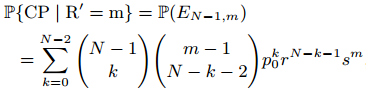
\includegraphics[width = 0.80\textwidth]{figures/cp.png}
	\end{subfigure}%
	\begin{subfigure}{0.50\textwidth}
	  \centering
	  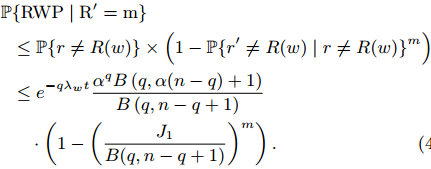
\includegraphics[width = 0.80\textwidth]{figures/rwp.png}
	\end{subfigure}
  \end{figure}
\end{frame}
%%%%%%%%%%%%%%%
\begin{frame}{PA2AM 量化分析}
  \begin{figure}
	\begin{subfigure}{0.40\textwidth}
	  \centering
	  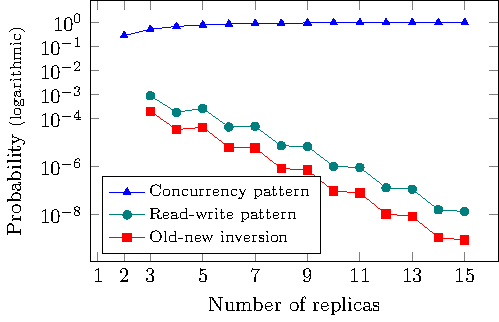
\includegraphics[width = 0.80\textwidth]{figures/oni-pgfplot.pdf}
	  \caption{数值结果.}
	\end{subfigure}%
	\begin{subfigure}{0.60\textwidth}
	  \centering
	  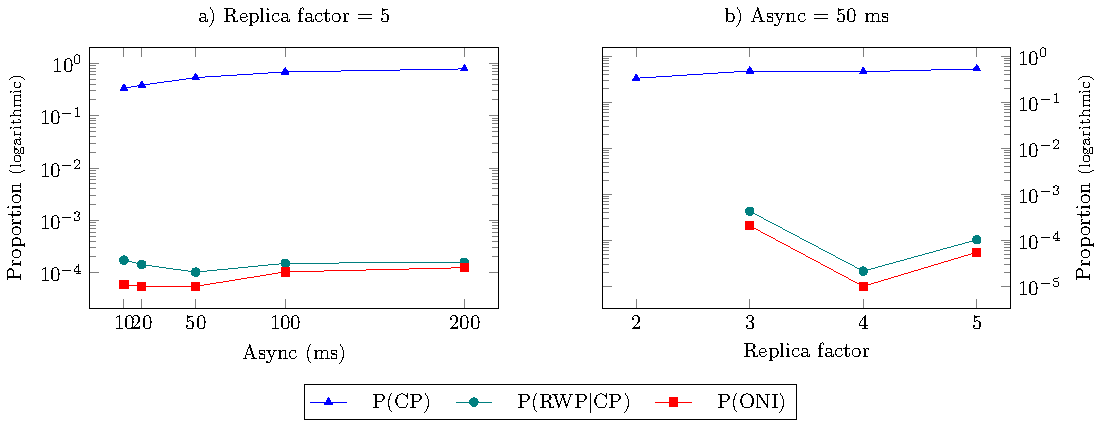
\includegraphics[width = 0.95\textwidth]{figures/experiment-oni-pgfplot.pdf}
	  \caption{实验结果.}
	\end{subfigure}
  \end{figure}

  \only<2->{
  \begin{cobservation}[观察一]
	从概率角度讲, PA2AM 算法极少违反 atomicity 一致性.
  \end{cobservation}
  }

  \only<3->{
  \begin{cobservation}[观察二]
	与经常发生的并发模式相比, 读写模式起主导作用。
  \end{cobservation}
}
\end{frame}
%%%%%%%%%%%%%%%
\begin{frame}{PA2AM vs. 弱一致性模型}
  \begin{figure}
	\begin{subfigure}{0.50\textwidth}
	  \centering
	  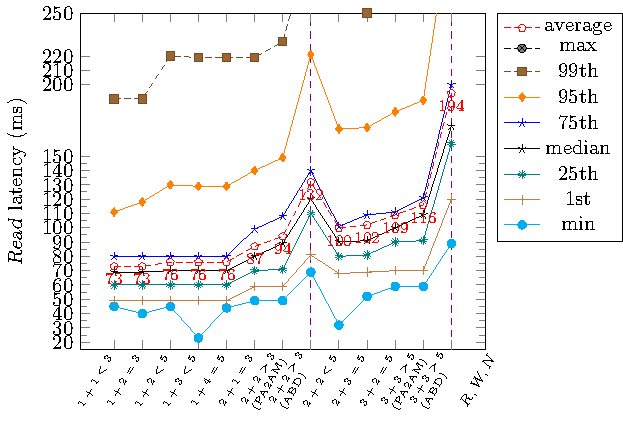
\includegraphics[width = 0.85\textwidth]{figures/rwn-2am-read-latency-quantiles.pdf}
	  \caption{读操作延迟对比.}
	\end{subfigure}%
	\begin{subfigure}{0.50\textwidth}
	  \centering
	  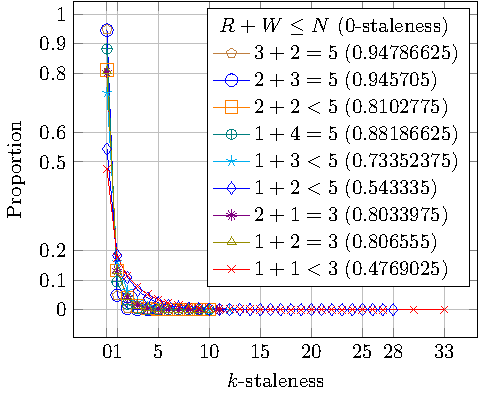
\includegraphics[width = 0.70\textwidth]{figures/rwn-maj.pdf}
	  \caption{$k$-陈旧度对比.}
	\end{subfigure}
	\caption{PA2AM 与 eventual consistency (RWN-Maj 协议) 对比结果.}
  \end{figure}

  \vspace{-0.50cm}
  \begin{table}[]
  \renewcommand{\arraystretch}{1.3}
  \centering
  \caption{不同 $R,W,N$ 配置下, RWN-All 执行中具有不同陈旧度的读操作的比率.}
  \label{tbl:rwn-all-staleness}
  \resizebox{\textwidth}{!}{%
  \begin{tabular}{|c||c|c|c|c||c|c|c|c|c|c|c|}
  \hline
  {\bfseries \# replicas} & \multicolumn{4}{c||}{\bfseries replica factor = 3 ($400,000$
    \textsl{read} operations)} & \multicolumn{7}{c|}{\bfseries replica factor = 5 ($800,000$
    \textsl{read} operations)} 
  \\ \hline
  {\bfseries $R,W,N$} % \textrm{R}+\textrm{W} $\boldsymbol{\le}$ \textrm{N}}  
  & $1+1<3$	& $1+2=3$	& $2+1=3$	& $2+2>3 \;(\text{PA2AM})$ 
  & $1+2<5$ 	& $1+3<5$ 	& $1+4=5$	& $2+2<5$ 	& $2+3=5$    & $3+2=5$     & $3+3>5 \;(\text{PA2AM})$     
  \\ \hline \hline
  {\boldmath $\max k$}          & $6$      & $4$ 	& $2$    &  {\boldmath $1$}
  & $2$	& $2$      	& $2$	   & $2$	& $2$	 &  $2$     & {\boldmath $1$}
  \\ \hline
  {\bfseries $\sum_{k \ge 1}$-staleness}       & $0.0084125$      & $0.000315$ 	&  $0.0004675$	&
  {\boldmath $0.000085$}
  	&  $0.00377875$	&  $0.002755$	&  $0.00406$     & $0.0027225$      & $0.0020275$     & $0.002255$      
	&  {\boldmath $0.0003525$}
  \\ \hline
  \end{tabular}%
}
\end{table}

\end{frame}
%%%%%%%%%%%%%%%
\begin{frame}{PA2AM 的意义}
  \mdf{red}{blue}{PA2AM 可作为数据一致性/访问延迟权衡的一种可行选项}{teal}{
	\begin{enumerate}
	  \item 既 {\small (在统计意义上)} 满足强一致性模型对数据一致性的高标准
	  \item 又具有弱一致性模型的性能优势
    \end{enumerate}
  }
\end{frame}
%%%%%%%%%%%%%%%
